\documentclass[a4paper]{article}

\usepackage{natbib}
\usepackage[english]{babel}
\usepackage[utf8]{inputenc}
\usepackage{amsmath}
\usepackage{graphicx}
\usepackage[colorinlistoftodos]{todonotes}

\usepackage{tikz}
\usetikzlibrary{math,fpu,calc,fit,mindmap,backgrounds,positioning}

\usepackage{xspace}
\newcommand{\eg}{e.g.\xspace}
\newcommand{\etal}{et al.\xspace}
\newcommand{\ie}{i.e.\xspace}
\newcommand{\etc}{etc.\xspace}
\newcommand{\vs}{\textit{vs.}\xspace}

\title{From Social Attention to Social Modelling in Robotics:\\ The Robotic Social Awareness Model}

\author{Séverin Lemaignan}

\date{\today}

\begin{document}
\maketitle

\begin{abstract}
Abstract goes here
\end{abstract}

\section{What do we aim for?}

Human social dynamics rely upon the ability to effectively attribute beliefs,
goals and percepts to other people. This set of meta-representational abilities
shapes what is called a theory of mind (ToM) or the ability to mentalize, and
leads to mutual modelling: the reciprocal ability to establish a mental model of
the other. This lays at the core of human interactions: normal human social
interactions depend upon the recognition of other sensory perspectives, the
understanding of other mental states, and the recognition of complex non-verbal
cues of attention and emotional state. As such, adapting and transferring these
cognitive skills to social robots is an important research objective.


Understanding and predicting one's behaviour.


\subsection{Surface Alignment vs Deep Grounding}

\citet{pickering2006alignment} argue that mutual understanding
starts mostly with a \emph{superficial alignment} at the level of the linguistic
representations, due to priming mechanisms, and that this local alignment may --
in some cases -- lead to a \emph{global alignment} of the semantic level
(\emph{deep grounding}).  For these authors, the convergence in dialogue, and
even the repair of some misunderstandings, is explained by this mimetic behavior
more than by a monitoring of each other's knowledge:

\begin{quote}
[\ldots] interlocutors do
not need to monitor and develop full common ground as a regular, constant
part of routine conversation, as it would be unnecessary and far too costly.
Establishment of full common ground is, we argue, a specialized and
non-automatic process that is used primarily in times of difficulty (when
radical misalignment becomes apparent).~\citep[p.179]{pickering2006alignment}
\end{quote}

\subsection{Theory of Mind}

In~\cite{scassellati2002theory}, Scassellati gave
an initial account of Leslie's and Baron-Cohen's respective models of the
emergence of a theory of mind (we discuss them below) from the perspective of
robotics, but reported implementation work was limited to simple perceptual
precursors (like face detection or color saliencies detection). Since then,
research in this field has been focused on applications relying on Flavell's
\emph{Level 1}~\cite{flavell1977development} perspective-taking, \ie
perspective-taking that only requires perceptual abilities (``\emph{I see (you do
not see the book)}''), and actually mostly limited to visual perception (relevant
work include Breazeal~\cite{breazeal2006using}, Trafton~\cite{Trafton2005} and
Ros~\cite{Ros2010}).

Based on perspective taking \emph{Level 1} alone, Breazeal
\etal\cite{breazeal2009embodied} and Warnier \etal\cite{warnier2012when}
successfully tackled the classical hallmark of theory of mind, the false belief
experiment (also known as the ``Sally and Anne'' experiment,
Figure~\ref{false-beliefs}, introduced by~\cite{wimmer1983beliefs}, original
experimental setting by~\cite{baron1985does}). They demonstrated complete
human-robot interaction scenarios where robots recognize and handle false belief
situations in dyadic or triadic interactions, and exhibit helping behaviours
that account for the missing/false beliefs of the human partners.


\section{A Cognitive Model of Social Awareness for Robots}

\subsection{The Attention Schemata Theory}

Our approach draws form the \emph{Attention Schemata Theory}, proposed by
Grazino~\cite{graziano2013consciousness}.

What awareness can do? ``the brain \emph{does} attention, but \emph{knows}
awareness'': as such, ``awareness can in principle be verbally reported''.



\subsection{Associative Memory Network}


In particular, used for behavioural alignment

\subsection{The Robotic Social Awareness Model}

Associative Memory as an Informational Proxy for the Attention System


\begin{enumerate}
    \item Perceptual inputs feed in an associative memory
    \item the resulting set of pre-activated units is labelled as the current
        \emph{focus of attention}
    \item According to the Attention Schemata Theory, by \emph{explicitely}
        labelling these units as being attended, we make the robot \emph{aware}
        of the corresponding phenomenons.
\end{enumerate}

\section{Attention}

Modelled as a \emph{Biased Competition Model of
Attention}~\cite{desimone1995neural}.
Implemented using a particular \emph{Associative Memory Network} with an
additional top-down biasing mechanism.


\begin{figure}
    \centering
        \resizebox{0.7\linewidth}{!}{%
        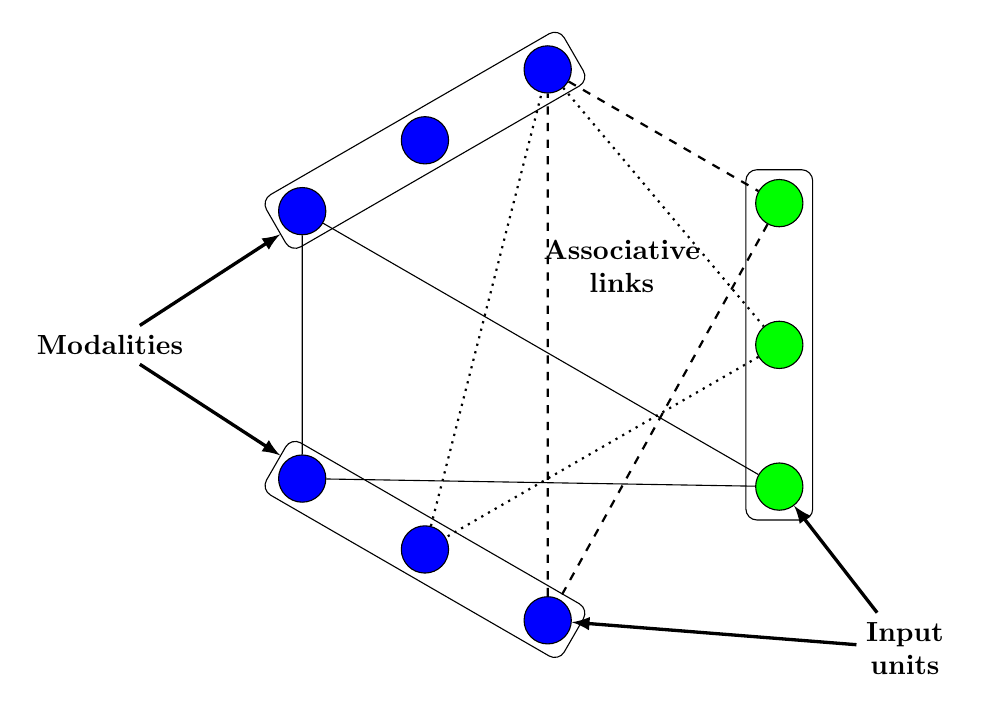
\begin{tikzpicture}[
                >=latex,
                every edge/.style={draw, very thick},
                every node/.style={font=\bf,align=center},
                input/.style={draw,circle, inner sep=0pt,minimum size=0.6cm}
            ]

            % draw the units
            \foreach \x [count=\xi] in {0, 120, 240}
                \foreach \y [count=\yi] in {-.6, 0, .6}
                    %\node[input, ball color=orange!\x!blue] at ($(\x:3)!\y!90:(0,0)$) (i\xi\yi) {};
                    \node[input, fill=blue!\x!green] at ($(\x:3)!\y!90:(0,0)$) (i\xi\yi) {};

            \node[draw,rounded corners, fit=(i11)(i12)(i13)] (modA) {};
            \node[draw,rounded corners, rotate fit=120,fit=(i21)(i22)(i23)] (modB) {};
            \node[draw,rounded corners, rotate fit=60,fit=(i31)(i32)(i33)] (modC) {};

            \node at (180:5.5) {Modalities} edge[->] (modB) edge[->] (modC);
            \node at (-40:6) {Input\\units} edge[->] (i13) edge[->] (i31);

            \path[draw,dashed, thick]  (i23) -- (i11) -- (i31) -- (i23);
            \path[draw,dotted, thick] (i23) -- (i12) -- (i32) -- (i23);
            \path[draw] (i21) -- (i13) -- (i33) -- (i21);

            \node at (1,1) {Associative\\links};
        \end{tikzpicture}
    }

    \caption{Associative Memory Network}
    \label{blabla}
\end{figure}



\subsection{Biasing Mechanisms}

Biasing competition~\cite{beck2009top}

The bottom-up biasing mechanism follows naturally from the structure of the
associatve memory model: a strong and long activation of a perceptual input
leads to the activation of the corresponding unit in the memory network and the
suppression of competing inputs.

The top-down mechanism is to be invented :-)
It should enable high-level decisional processes to effectively suppress (or
reinforce) units. The \emph{nature} and \emph{representation} of these
high-level processes is unclear, but might be of symbolic nature.



\section{Social Attention}

What do we call the \emph{attention state} of a partner?


Grazino~\cite{graziano2013consciousness}: ``the mental machinery to model
someone else attentional state is the same as the one used for oneself.''
``In both case, the purpose is understanding and predicting one's behaviour.''

Cues from which we reconstruct someone else's attentional state (from Graziano):
\begin{itemize}
    \item gaze direction
    \item facial expression
    \item body language
    \item prior knowledge of person
    \item location of salient objects
\end{itemize}


\section{The functional pre-requisites for social robots}

\subsection{Social Assessment}
\subsubsection{Gaze direction}
\subsubsection{Facial and body expressions}
\subsubsection{Gestures}

\subsection{Situation Assessment}

Including saliency information

\section{Evaluation of the Model}

\subsection{Does it perform as well as Symbolic Architectures?}
\subsection{Comparison with Symbolic Situation Assessment}




\bibliographystyle{plain}
\bibliography{biblio}

\end{document}
